\chapter{Kernel 4-bit bất biến theo số hàng cho giải mã suy đoán exact}\label{chap:kernel}

\providecommand{\code}[1]{\texttt{\detokenize{#1}}}
\providecommand{\ci}[3]{#1 [#2,\,#3]}

Chương~\ref{chap:b2} xây dựng vòng giải mã exact B2 bằng cách gọi từng hàng các toán tử nhạy với hình dạng. Cách đó giữ đúng chuỗi của bitsandbytes gốc nhưng bỏ phần lớn lợi ích của việc kiểm tra theo khối: trọng số được đọc lại cho mỗi hàng. Chương này đi theo hướng ngược lại, trả lời RQ6: \emph{có thể thiết kế các kernel 4-bit mà kết quả của từng hàng không phụ thuộc vào số hàng $M$ trong khối, sao cho kiểm tra theo khối vừa exact vừa thực sự đọc trọng số một lần?} Cái giá phải trả là tham chiếu exact không còn là bitsandbytes gốc mà là chính bộ kernel mới chạy ở $M{=}1$; mục~\ref{sec:k-ref} đo sự khác biệt này.

\section{Vấn đề: kernel đổi chiến lược theo $M$}\label{sec:k-problem}
Trên một GPU, thư viện chọn kích thước tile, hệ số chia chiều rút gọn (split-K) hoặc cả kernel khác nhau tùy số hàng. Hệ quả là cùng một hàng kích hoạt cho kết quả khác từng bit khi nằm trong khối $M{=}1$ hay $M{=}4$. Bảng~\ref{tab:k-audit} tóm tắt phép kiểm toán theo toán tử trên bitsandbytes 0.50.0 (RTX 4050, sm\_89): phép chiếu NF4 ổn định đến $M{=}3$ rồi lệch khoảng $13$--$15\%$ phần tử từ $M{\ge}4$, khớp với việc bitsandbytes đổi kernel ở $M{=}4$; attention (SDPA) lệch $3.6$--$19.2\%$ phần tử ở mọi $M$, LM head lệch $0$--$0.19\%$, RMSNorm lệch ở một số mô hình. Ngưỡng $M{=}4$ chỉ đo trên phiên bản và GPU này; bản 0.50.1/0.50.2 đổi cách chọn kernel nên không suy rộng được.

\begin{table}[t]
\centering\small
\caption{Độ lệch từng bit so với chạy từng hàng, bitsandbytes 0.50.0 NF4, GSM8K, 960 hàng mỗi ô. ``Proj'': tỷ lệ phần tử sai của các phép chiếu NF4; RMSNorm là số phần tử sai.}\label{tab:k-audit}
\begin{tabular}{@{}lrrrrr@{}}
\toprule
Mô hình & $M$ & Proj & RMSNorm & LM head & SDPA\\\midrule
Qwen2.5-3B & 2 & 0\% & 60 & 0.193\% & 18.6\%\\
Qwen2.5-3B & 3 & 0\% & 87 & 0.193\% & 18.6\%\\
Qwen2.5-3B & 4 & 12.96\% & 244 & 0.193\% & 18.6\%\\
Qwen2.5-3B & 8 & 12.96\% & 199 & 0.193\% & 18.6\%\\
Qwen2.5-1.5B & 4 & 13.85\% & 92 & 0.109\% & 18.3\%\\
Qwen2.5-0.5B & 4 & 14.27\% & 0 & 0.000\% & 3.6\%\\
OLMo-2-1B & 4 & 15.42\% & 189 & 0.048\% & 17.4\%\\
Phi-3.5-mini & 4 & 14.79\% & 459 & 0.083\% & 19.2\%\\
\bottomrule
\end{tabular}
\end{table}

Hệ quả cuối-cuối: PLD ngây thơ (kiểm tra theo khối, kernel gốc) rời khỏi quỹ đạo greedy tuần tự ở $26$--$82\%$ số chuỗi trên 15 ô (5 mô hình $\times$ 3 tập, 50 prompt mỗi ô; tới $92\%$ trên một tập CNN/DM độc lập), còn một mô hình nháp thật (Qwen2.5-0.5B nháp cho 3B, $K{=}2,4,6$) lệch $34$--$38\%$ trên GSM8K và $64$--$66\%$ trên CNN/DM. Chạy từng hàng đưa cả hai về $0$ lệch (\cref{fig:k-naive}). Quan sát định tính rằng kiểm tra theo khối trên backend lượng tử hóa làm đổi logit và đổi argmax đã được báo cáo trên Metal \cite{chordiya2026lossless}; đóng góp ở đây là đo theo từng toán tử trên CUDA và phần sửa.

\begin{figure}[t]
\centering
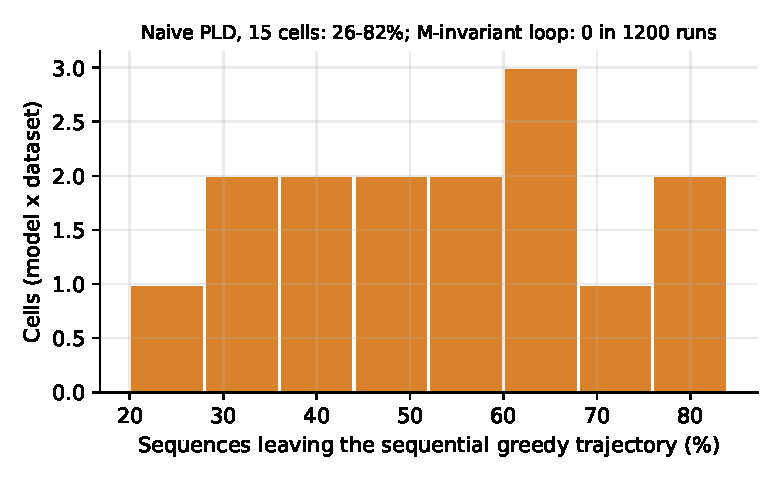
\includegraphics[width=0.6\textwidth]{images/kernel_naive_divergence.pdf}
\caption{Phân bố tỷ lệ chuỗi lệch quỹ đạo greedy tuần tự của PLD ngây thơ trên 15 ô (mô hình $\times$ tập dữ liệu).}\label{fig:k-naive}
\end{figure}

\section{Định nghĩa exact và tham chiếu}\label{sec:k-ref}
Gọi $\mathcal K$ là một bộ kernel cố định và $R_{\mathcal K}$ là giải mã greedy tuần tự dùng $\mathcal K$ với $M{=}1$ ở mọi bước. Một bộ giải mã suy đoán là \emph{exact theo $\mathcal K$} nếu với mọi prompt nó trả về đúng các token của $R_{\mathcal K}$ và để lại đúng các byte KV cache của $R_{\mathcal K}$. Ta \emph{không} đòi bằng greedy bitsandbytes gốc: đó là một bộ kernel khác.

Hai bộ kernel hợp lệ khác thứ tự cộng thì tách nhau. Phép đo trên Qwen2.5-3B (\cref{tab:k-ref}) cho thấy chuỗi từ tham chiếu bất biến giống hệt chuỗi bitsandbytes gốc ở chỉ $30\%$ ($n{=}50$) và $44\%$ ($n{=}150$) số prompt GSM8K, cùng cỡ với mức lệch của PLD ngây thơ. Độ chính xác tác vụ không bị phát hiện giảm: GSM8K $72\%$ so với $66\%$ ($n{=}50$, $5$ so với $2$ cặp bất đồng, trong nhiễu). Đây là kiểm tra không phát hiện sai khác, không phải chứng minh tương đương. Trên HumanEval ($n{=}100$, prompt thô, tối đa $384$ token) pass@1 là $61/100$ ở cả hai chế độ, với $3$ và $3$ bài bất đồng theo hai chiều; chuỗi token giống hệt ở $72/100$ prompt (mức giống cao hơn GSM8K vì đầu ra ngắn hơn). Con số $61\%$ thấp hơn mức công bố cho mô hình vì ta dùng prompt thô và cắt hoàn thành bằng quy tắc đơn giản, nên chỉ có ý nghĩa để so hai chế độ với nhau.

\begin{table}[t]
\centering\small
\caption{Tham chiếu bất biến so với greedy bitsandbytes gốc, Qwen2.5-3B NF4.}\label{tab:k-ref}
\begin{tabular}{@{}lrrr@{}}
\toprule
Phép đo & $n$ & Gốc & Bất biến\\\midrule
Chuỗi giống hệt (GSM8K) & 50 & \multicolumn{2}{c}{$15$ ($30\%$)}\\
Chuỗi giống hệt (GSM8K, ext150) & 150 & \multicolumn{2}{c}{$66$ ($44\%$)}\\
Độ chính xác GSM8K & 50 & $33$ ($66\%$) & $36$ ($72\%$)\\
Chuỗi giống hệt (HumanEval) & 100 & \multicolumn{2}{c}{$72$ ($72\%$)}\\
pass@1 HumanEval & 100 & $61$ ($61\%$) & $61$ ($61\%$)\\
\bottomrule
\end{tabular}
\end{table}

\section{Thiết kế kernel bất biến}\label{sec:k-design}
\paragraph{Nguyên tắc.} Phần tử đầu ra $(m,n)$ được tính bởi cùng một dãy lệnh bất kể $M$ và các hàng khác. Có bốn quy tắc: (i) đệm số 0 khối hàng về kích thước cố định $M_P$; (ii) thứ tự rút gọn theo $K$ cố định; (iii) không split-K, không atomics, không tự điều chỉnh (autotune); (iv) không có phụ thuộc dữ liệu giữa các hàng. Bất biến được kiểm bằng thực nghiệm (hàng chục nghìn hàng mỗi kernel); chương này không chứng minh hình thức. \cref{fig:k-principle} minh họa nguyên tắc.


\begin{figure}[t]
\centering
\begin{tikzpicture}[x=1cm,y=1cm,font=\small]
  % input rows
  \foreach \i/\lab in {0/$x_0$,1/$x_1$,2/$x_2$} { \draw[fill=blue!15] (0,-\i*0.6) rectangle (2.4,-\i*0.6-0.5); \node at (1.2,-\i*0.6-0.25) {\lab}; }
  \foreach \i in {3,4,5} { \draw[dashed,fill=gray!10] (0,-\i*0.6) rectangle (2.4,-\i*0.6-0.5); \node at (1.2,-\i*0.6-0.25) {0}; }
  \node[align=center] at (1.2,0.45) {khối $M{=}3$ hàng\\đệm $0$ tới $M_P$};
  \draw[->,thick] (2.6,-1.5) -- (3.6,-1.5);
  % kernel
  \draw[fill=orange!15] (3.7,-3.2) rectangle (7.7,0.3);
  \node[align=center] at (5.7,-0.4) {\textbf{kernel bất biến}};
  \node[align=left,font=\footnotesize] at (5.7,-1.8) {thứ tự rút gọn $K$ cố định\\không split-K / atomics\\không autotune\\mỗi hàng độc lập};
  \draw[->,thick] (7.9,-1.5) -- (8.9,-1.5);
  % outputs
  \foreach \i/\lab in {0/$y_0$,1/$y_1$,2/$y_2$} { \draw[fill=green!15] (9.0,-\i*0.6) rectangle (11.4,-\i*0.6-0.5); \node at (10.2,-\i*0.6-0.25) {\lab}; }
  \node[align=center,font=\footnotesize] at (10.2,-2.4) {$y_i$ giống từng bit\\với chạy $M{=}1$};
\end{tikzpicture}
\caption{Nguyên tắc thiết kế: khối $M$ hàng được đệm $0$ tới kích thước cố định $M_P$ và đi qua cùng một dãy lệnh; kết quả mỗi hàng không phụ thuộc $M$.}\label{fig:k-principle}
\end{figure}

\paragraph{LM head.} Kernel Triton dùng \code{tl.dot} trên khối $16$ hàng (đệm $0$), fp16/bf16 $\to$ fp32, $K$ chia khối $128$ theo thứ tự cố định. Kết quả bằng từng bit với GEMM cuBLAS khi $M{\ge}2$ nhưng không bằng đường gemv của cuBLAS ở $M{=}1$ ($1.2\%$ phần tử khác); đây là lý do tham chiếu không trùng bitsandbytes gốc. Chi phí $3.42$~ms so với $3.34$~ms của cuBLAS ở $M{=}1$ ($1.02\times$) và gần như không đổi theo $M{=}1..8$; chạy từng hàng ba lần tốn $10.8$~ms.

\paragraph{Attention.} Kernel Triton split-KV với các đoạn khóa tuyệt đối (256 khóa, tile 64): mỗi đoạn tính softmax trực tuyến riêng, các kết quả riêng được gộp theo thứ tự đoạn tăng dần. Đoạn bị che hoàn toàn là phép không (no-op) chính xác, nên kết quả một hàng không phụ thuộc vào số hàng hay vị trí sau nó. Ở chế độ CUDA graph, độ dài tiền tố là một số \code{int32} trên thiết bị. GQA dùng K/V gọn. Ở $M{=}3$ nhanh hơn SDPA có mặt nạ $5$--$25$ lần.

\paragraph{RMSNorm.} Mỗi chương trình xử lý đúng một hàng.

\paragraph{GEMM NF4.} Kernel CUDA C++ dùng bố cục bitsandbytes (nibble cao trước, blocksize $64$, absmax lượng tử hóa kép). Một warp xử lý $R$ hàng đầu ra và $M_P$ hàng kích hoạt; trọng số được đọc và giải lượng tử một lần cho mọi hàng, đây là nơi có lợi ích so với chạy từng hàng. Mỗi lane xử lý $32$ phần tử $K$ mỗi bước $1024$ phần tử, cộng dồn \code{fmaf} theo thứ tự cố định rồi rút gọn xor-butterfly. Các biến thể $M_P\in\{1,2,4,8\}$ và $R\in\{1,2,4,8\}$ cho cùng từng bit trên mỗi hàng ($0$ lệch trên $7000$ hàng). Hai phiên bản Triton đầu chậm hơn bitsandbytes $4$--$20$ lần nên bị bỏ.

\begin{algorithm}[t]
\caption{Kernel GEMM NF4 bất biến theo $M$ (một warp).}\label{alg:nf4}
\begin{algorithmic}[1]
\Require $R$ hàng trọng số NF4, $M\le M_P$ hàng kích hoạt (đệm $0$ tới $M_P$)
\Ensure $Y[m,r]$ với $m<M$, độ lớn không phụ thuộc $M$
\For{$k_0 = 0,1024,2048,\dots$} \Comment{thứ tự cố định}
  \State mỗi lane nạp $32$ nibble của mỗi hàng trọng số, giải lượng tử một lần
  \For{$m=0..M_P-1$, $r=0..R-1$}
    \State $acc[m,r] \gets \mathrm{fmaf}(x[m,k], w[r,k], acc[m,r])$ theo $k$ tăng dần
  \EndFor
\EndFor
\State rút gọn $acc[m,r]$ qua $32$ lane bằng xor-butterfly cố định
\State cộng bias (fp32) và làm tròn về dtype đầu ra
\end{algorithmic}
\end{algorithm}

\paragraph{Một lỗi mà kiểm tra ``exact'' không bắt được.} Bản đầu của kernel NF4 đọc bias fp16 như bf16 và cho đầu ra vô nghĩa trong mô hình thật, nhưng vẫn ``exact'' $100\%$ vì mọi cách chạy đều sinh cùng một chuỗi lặp vô nghĩa. Lỗi chỉ lộ khi đọc văn bản sinh ra; đã sửa (bias chuyển sang fp32) và so từng lớp với ma trận giải lượng tử fp32 trên kích hoạt thật. Bài học: kiểm tra exact phải đi kèm kiểm tra văn bản hoặc độ chính xác tác vụ. Mọi số liệu tốc độ trong chương đều sinh sau bản sửa.

\begin{table}[t]
\centering\small
\caption{Kiểm chứng bất biến theo $M$ (số hàng lệch / tổng số hàng kiểm).}\label{tab:k-inv}
\begin{tabular}{@{}lrl@{}}
\toprule
Kernel & Hàng kiểm & Lệch\\\midrule
LM head (5 hình dạng) & 27\,000 & 0\\
Attention (Qwen 3B, 1.5B, 0.5B; ngữ cảnh $128$--$3000$) & $3\times 6300$ & 0\\
Attention MHA $32/32$ & 2\,100 & 0\\
GEMM NF4 (mọi biến thể $M_P$, $R$) & 7\,000 & 0\\
\bottomrule
\end{tabular}
\end{table}

\section{Chi phí một bước giải mã}\label{sec:k-cost}
Thời gian một bước giải mã đầy đủ trong CUDA graph (Qwen2.5-3B): $M{=}1$ $15.0$~ms (bitsandbytes $16.3$), $M{=}3$--$4$ $17.7$~ms (bitsandbytes $21.2$ đến $31.5$), $M{=}5$--$6$ $23.6$~ms (bitsandbytes $31$) (\cref{fig:k-step}). Kernel GEMM chiếm $9.2$~ms ở $M{=}1$, chậm hơn \code{gemm_4bit_simt} của bitsandbytes ($8.9$~ms) khoảng $3\%$ nhưng nhanh rõ ở $M{\ge}3$. Nghĩa là bước kiểm tra $M{=}3$ chỉ đắt hơn bước $M{=}1$ khoảng $18\%$, đúng điều kiện để giải mã suy đoán có lợi.

\begin{figure}[t]
\centering
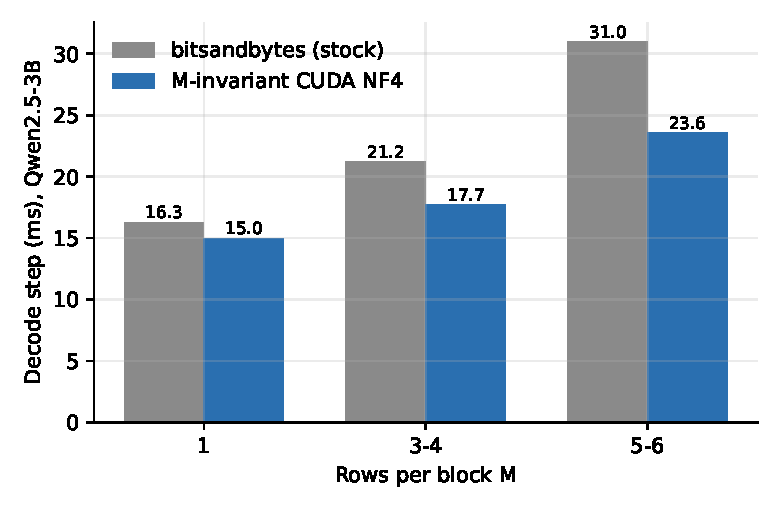
\includegraphics[width=0.55\textwidth]{images/kernel_step_time.pdf}
\caption{Thời gian một bước giải mã trong CUDA graph, Qwen2.5-3B NF4, theo số hàng của khối.}\label{fig:k-step}
\end{figure}

\section{Vòng giải mã exact trên CUDA graph}\label{sec:k-loop}
PLD đề xuất tối đa $K{=}2$ token (n-gram $3$); khối $M\le 3$ hàng được kiểm tra bằng các kernel bất biến trong một lần phát lại CUDA graph; token được chấp nhận được commit, hàng bị loại được quay lui bằng cách đặt lại độ dài của static cache (\code{cumulative_length.fill_(n)}); tensor tiền tố của attention được cập nhật trước mỗi lần phát lại. Vì mọi kernel bất biến theo $M$, byte KV đã commit bằng của giải mã tuần tự, điều ta kiểm trực tiếp.

\begin{algorithm}[t]
\caption{Vòng PLD exact với kernel bất biến.}\label{alg:loop}
\begin{algorithmic}[1]
\Require prompt, tham chiếu $R_{\mathcal K}$, $K{=}2$
\State prefill bằng kernel bất biến; $n \gets$ độ dài tiền tố
\While{chưa EOS và chưa đủ token}
  \State $d \gets$ tra n-gram (tối đa $K$ token) \Comment{có thể rỗng}
  \State chạy khối $1{+}|d|$ hàng bằng đồ thị CUDA ($M\in\{1,2,3\}$)
  \State $j \gets$ số token nháp khớp argmax; commit $j{+}1$ token
  \State \code{cumulative_length.fill_(n + j + 1)}; $n \gets n+j+1$ \Comment{quay lui KV}
\EndWhile
\end{algorithmic}
\end{algorithm}

\section{Kết quả đầu-cuối}\label{sec:k-results}
\paragraph{Thiết lập.} RTX 4050 Laptop 6~GB, Triton 3.6.0, nvcc 12.8, bitsandbytes 0.50.0, greedy, batch 1, $128$ token mới, $K{=}2$, n-gram $3$. Baseline là giải mã $M{=}1$ exact dùng cùng kernel bất biến trong CUDA graph, cùng phiên và cùng prompt. ``Exact'' là token sinh ra \emph{và} KV đã commit bằng từng bit với $R_{\mathcal K}$.

\begin{table}[t]
\centering\small
\caption{Vòng PLD exact so với baseline $M{=}1$ cùng kernel. Tăng tốc theo prompt là trung vị [min, max]. Cận trên Wilson $95\%$ của tỷ lệ lệch: $1.9\%$ ($n{=}200$), $3.7\%$ ($n{=}100$).}\label{tab:k-speed}
\begin{tabular}{@{}lrrrrrl@{}}
\toprule
Ô & Prompt & Exact & Base & PLD & Tăng & Theo prompt\\\midrule
Qwen2.5-3B GSM8K & 200 & 200/200 & 61.2 & 71.8 & $1.17\times$ & $1.18$ [1.01, 1.40]\\
Qwen2.5-3B HumanEval & 100 & 100/100 & 58.9 & 77.6 & $1.32\times$ & $1.32$ [1.01, 2.22]\\
Qwen2.5-3B CNN/DM & 100 & 100/100 & 58.7 & 70.7 & $1.21\times$ & $1.21$ [0.98, 1.54]\\
Qwen2.5-1.5B GSM8K & 100 & 100/100 & 97.1 & 115.6 & $1.19\times$ & $1.18$ [1.01, 1.53]\\
Qwen2.5-0.5B GSM8K & 100 & 100/100 & 196.0 & 241.9 & $1.23\times$ & $1.22$ [1.05, 1.67]\\
OLMo-2-1B GSM8K & 100 & 100/100 & 136.2 & 155.1 & $1.14\times$ & $1.13$ [1.02, 1.37]\\
Phi-3.5-mini GSM8K & 100 & 100/100 & 72.7 & 85.9 & $1.18\times$ & $1.18$ [1.05, 1.41]\\
Llama-3.2-1B GSM8K & 100 & 100/100 & 135.1 & 171.5 & $1.27\times$ & $1.26$ [1.04, 2.15]\\
Llama-3.2-3B GSM8K & 100 & 100/100 & 62.9 & 78.2 & $1.24\times$ & $1.21$ [1.05, 2.20]\\
Mistral-7B GSM8K & 100 & 100/100 & 38.1 & 45.8 & $1.20\times$ & $1.20$ [1.07, 1.50]\\
Mistral-7B HumanEval & 100 & 100/100 & 35.5 & 44.1 & $1.24\times$ & $1.21$ [1.00, 1.94]\\
\bottomrule
\end{tabular}
\end{table}

Tổng cộng $1200$ cặp (prompt, mô hình) trên $8$ mô hình (năm họ Qwen2.5, OLMo-2, Phi-3.5, Llama-3.2 và Mistral; GQA và MHA; $head\_dim$ $64$, $96$ và $128$): $0$ lệch về token và KV; các lần chạy lặp (cùng phiên so sánh, kiểm tra EOS, kiểm tra phiên bản) cũng đều exact. Tăng tốc $1.14$--$1.32\times$; chỉ một prompt (CNN/DM) chậm hơn baseline ($0.98\times$) (\cref{fig:k-cells}). Phi-3.5 cần hai chỉnh sửa hạ tầng chứ không đổi kernel: kernel attention được mở rộng cho $head\_dim$ $96$ (đệm lên $128$ trong kernel bằng mặt nạ, $0$ lệch trên $700$ hàng, bốn kernel cũ vẫn $0$ lệch), RoPE LongRoPE được cố định ở chế độ hệ số ngắn (đúng với ngữ cảnh dưới $4096$ token, vì bản gốc chọn hệ số bằng một phép đồng bộ dữ liệu làm hỏng CUDA graph), và cache dùng lớp tĩnh thông thường thay cho lớp cửa sổ trượt (cửa sổ $262144$ lớn hơn ngữ cảnh, lớp cửa sổ trượt giữ độ dài bằng số nguyên Python nên không quay lui được). Lần chạy đầu của Phi-3.5 trước khi sửa lớp cache cho tốc độ cao bất thường ($1.74\times$) nhưng không exact; cờ exact đã phát hiện được lỗi này. Hai mô hình Llama-3.2 và Mistral-7B-Instruct-v0.3 (bản sao không cần token của unsloth; Mistral là mô hình $7$B đầu tiên, tải sẵn dạng NF4 và vừa GPU $6$~GB với cache ngắn) chạy không cần sửa gì. Trên Mistral-7B, một bước giải mã $M{=}1$ tốn khoảng $26$--$28$~ms, gần gấp đôi mô hình $3$B, nhưng mức tăng của PLD ($1.20$--$1.24\times$) tương đương các mô hình nhỏ; ở HumanEval, tăng tốc chỉ trên $55$ prompt không có EOS là $1.28\times$. Baseline $M{=}1$ bất biến còn nhanh hơn baseline graph kernel gốc ($62.4$ so với $57.8$~tok/s trên GSM8K).

\begin{figure}[t]
\centering
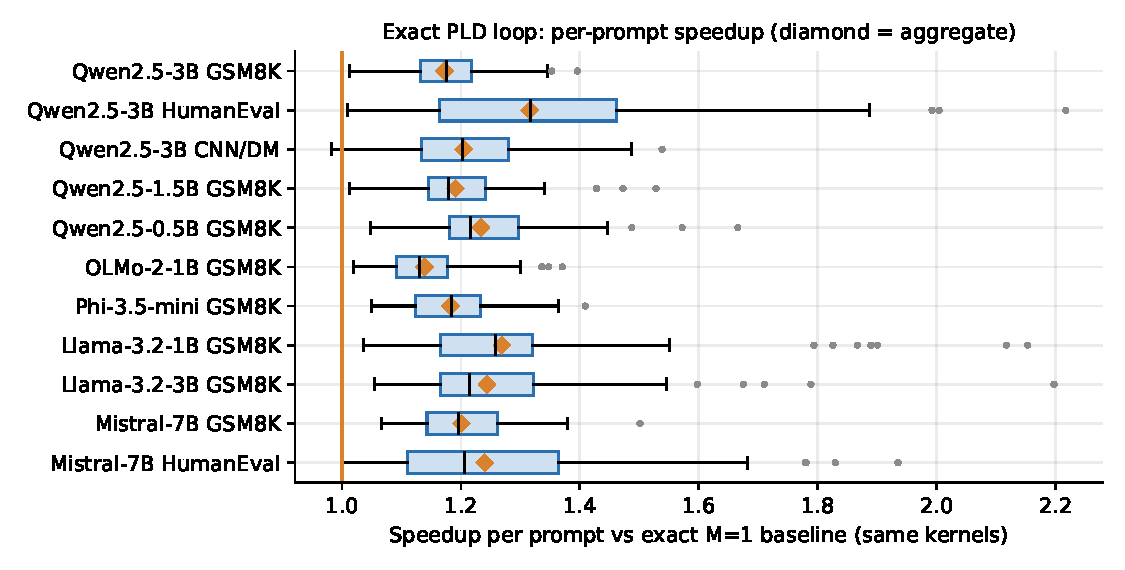
\includegraphics[width=0.85\textwidth]{images/kernel_speedup_cells.pdf}
\caption{Phân bố tăng tốc theo prompt của vòng PLD exact so với baseline $M{=}1$ cùng kernel.}\label{fig:k-cells}
\end{figure}

\paragraph{So với vòng exact cũ chạy từng hàng.} Cùng prompt, chạy liền nhau (vòng cũ, vòng mới, vòng cũ để đo trôi): với $100$ prompt mỗi tập, vòng mới đạt $79.0$ tok/s trên GSM8K so với $62.7$ và $61.2$ của vòng cũ ($1.26\times$ và $1.29\times$), $76.5$ so với $56.4$ và $57.0$ trên CNN/DM ($1.36\times$ và $1.34\times$), $81.9$ so với $58.9$ và $59.4$ trên HumanEval ($1.39\times$ và $1.38\times$); tất cả các lượt đều exact. Hai lần chạy vòng cũ lệch nhau nhiều nhất $2.4\%$, nên nhiễu giữa các phiên nhỏ hơn mức chênh. So với baseline $M{=}1$ bất biến cùng phiên, mức tăng trong các phiên này là $1.18\times$, $1.20\times$ và $1.31\times$ (nhanh hơn một chút so với Bảng~\ref{tab:k-speed} do phiên chạy khác nhau).

\paragraph{Ablation.} PLD với $K{=}4$ chậm hơn $K{=}2$ ($1.145\times$ so với $1.206\times$, 10 prompt). Tắt làm tròn trọng số hay thay tra bảng bằng phép tính chỉ đổi thời gian GEMM dưới $5\%$; ở $M{=}4$ kernel gần giới hạn số phép FMA, ở $M{=}1$ còn cách giới hạn băng thông khoảng $20\%$. Ước tính tối đa $10\%$ thời gian bước còn thu hồi được, tăng đều cho cả baseline lẫn vòng PLD nên gần như không đổi tỷ số tăng tốc.

\paragraph{Kiểm tra văn bản sau EOS.} Vòng sinh đúng $128$ token và không dừng ở EOS, nên với prompt có EOS sớm phần sau là văn bản lặp, thứ mà PLD đoán rất dễ và có thể làm tăng tốc cao hơn thực tế. Ta chạy lại sáu ô (100 prompt mỗi ô) ghi vị trí EOS đầu tiên của chuỗi tham chiếu: tỷ lệ prompt có EOS trong $128$ token là $0\%$ (Qwen-3B GSM8K), $26\%$ (HumanEval), $8\%$ (CNN/DM), $9\%$ (Llama-3B), $17\%$ (Llama-1B) và $15\%$ (Phi-3.5). Tăng tốc chỉ tính trên các prompt không có EOS lần lượt là $1.18$, $1.32$, $1.21$, $1.23$, $1.29$ và $1.19\times$, so với $1.18$, $1.32$, $1.20$, $1.24$, $1.27$ và $1.18\times$ khi tính mọi prompt (lệch dưới $2\%$); cả $600$ lượt chạy này đều exact. Văn bản sau EOS vì vậy không làm tăng số đo.

\section{Độ phụ thuộc vào phiên bản bitsandbytes}\label{sec:k-bnbver}
Kernel GEMM NF4 của ta chỉ dùng bố cục lượng tử hóa của bitsandbytes, không gọi kernel nhân của nó, nên bộ kernel không phụ thuộc cách bitsandbytes chọn kernel. Ngược lại, hành vi của đường gốc mà ta thay thế phụ thuộc phiên bản. Ta đo tỷ lệ phần tử khác từng bit giữa phép chiếu NF4 chạy cả khối $M$ hàng và chạy từng hàng, trên dữ liệu ngẫu nhiên với ba hình dạng của Qwen2.5-3B (\cref{tab:k-bnbver}): bitsandbytes 0.50.0 và 0.50.1 cho kết quả giống hệt nhau (ổn định đến $M{=}3$ và lệch $\approx60\%$ phần tử từ $M{\ge}4$), còn 0.49.2 (trước PR \#1949 thêm kernel GEMM 4-bit hợp nhất) lệch $\approx60\%$ ngay từ $M{=}2$. Nói cách khác ngưỡng $M{=}4$ chỉ là tính chất của 0.50.x; trên 0.49.2 ngay cả khối hai hàng cũng không an toàn. Bộ kernel bất biến vượt cả bốn kiểm tra đơn vị và vòng exact trên 20 prompt GSM8K với cả 0.49.2 và 0.50.1 ($20/20$ exact, tăng $1.19\times$ và $1.20\times$ so với baseline $M{=}1$ bất biến). Các tỷ lệ $\approx60\%$ lớn hơn $13$--$15\%$ ở Bảng~\ref{tab:k-audit} vì dữ liệu ngẫu nhiên fp16 khác kích hoạt thật; chỉ so sánh giữa các phiên bản mới có ý nghĩa.

\begin{table}[t]
\centering\small
\caption{Tỷ lệ phần tử NF4 khác từng bit giữa khối $M$ hàng và chạy từng hàng (stock bitsandbytes, hình dạng $11008{\times}2048$, dữ liệu ngẫu nhiên).}\label{tab:k-bnbver}
\begin{tabular}{@{}lrrrrr@{}}
\toprule
Phiên bản & $M{=}2$ & $M{=}3$ & $M{=}4$ & $M{=}8$ & $M{=}16$\\\midrule
0.49.2 & 60.5\% & 60.2\% & 60.2\% & 60.3\% & 60.4\%\\
0.50.0 & 0\% & 0\% & 60.2\% & 60.3\% & 60.4\%\\
0.50.1 & 0\% & 0\% & 60.2\% & 60.3\% & 60.4\%\\
\bottomrule
\end{tabular}
\end{table}

\section{Kết quả âm}\label{sec:k-neg}
\begin{itemize}[nosep]
\item \textbf{Mô hình nháp thần kinh.} Qwen2.5-0.5B bf16 nháp cho 3B NF4 ($K{=}2$) exact nhưng chỉ $0.66\times$ baseline: một bước nháp tốn khoảng $10$~ms so với $15$~ms của một bước đích. Tính từ số đo, ngay cả nháp nén NF4 cũng chỉ khoảng $0.87\times$, và nháp miễn phí bị chặn ở khoảng $1.36\times$. Với đích 4-bit $3$B đã rất rẻ trên GPU này, PLD là nguồn nháp phù hợp. Với đích $\ge7$B tình hình có thể khác nhưng chưa đo được.
\item \textbf{Tối ưu kernel} còn tối đa khoảng $10\%$ (mục trước).
\item Tiêu chí ban đầu ``$\ge1.15\times$ với mô hình nháp thật'' \emph{không đạt}; chỉ PLD đạt tăng tốc.
\end{itemize}

\section{Giới hạn và mối đe dọa tính hợp lệ}\label{sec:k-limits}
(i) Một GPU (RTX 4050 6~GB), mô hình tới $7$B (chỉ một mô hình $7$B, với cache ngắn), batch $1$, chỉ greedy; chưa chạy mô hình $\ge7$B hay GPU khác. (ii) Bất biến dựa vào cấu trúc kernel và thực nghiệm, không phải chứng minh, và phụ thuộc phiên bản trình biên dịch (Triton 3.6.0, nvcc 12.8); các kiểm tra bất biến và vòng exact (20 prompt) cũng đạt với bitsandbytes 0.49.2 và 0.50.1 (xem mục~\ref{sec:k-bnbver}), nhưng chỉ trên một GPU. (iii) Chưa thử họ kiến trúc nào ngoài Qwen2, OLMo-2, Phi-3 và Llama-3.2 (chưa có Gemma và mô hình MoE). (iv) Tăng tốc phụ thuộc mức PLD tìm được bản nháp: cao nhất ở HumanEval, thấp nhất ở OLMo-2. (v) So sánh độ chính xác với tham chiếu gốc còn nhỏ ($n{=}50$ trên GSM8K). (vi) Phi-3.5 chỉ được hỗ trợ trong chế độ ngữ cảnh $\le4096$ token (hệ số LongRoPE ngắn). (vii) Mọi prompt dùng văn bản thô (không dùng chat template). (viii) So sánh với LLM-42 và các công trình đồng thời mới ở mức đọc tài liệu.

\section{Tóm tắt chương}
Bộ kernel bất biến theo $M$ (LM head, attention, RMSNorm, GEMM NF4) cho phép kiểm tra theo khối exact theo bộ kernel của chính nó, và vòng PLD trên CUDA graph chạy nhanh hơn giải mã exact $M{=}1$ cùng kernel $1.14$--$1.32\times$ với $0$ lệch trong $1200$ cặp prompt-mô hình. Mức tăng là khiêm tốn, phụ thuộc workload và chỉ có với PLD; mô hình nháp thần kinh không có lợi trên đích $3$B. Tham chiếu exact là bộ kernel mới, khác bitsandbytes gốc ở phần lớn chuỗi nhưng không phát hiện giảm độ chính xác tác vụ ở cỡ mẫu nhỏ.

\paragraph{Mã nguồn.} \texttt{src/zassd/kernels/}, \texttt{scripts/wp*}, số liệu ở \texttt{results/kernels/}; kế hoạch và bản thảo bài báo ở \texttt{docs/PLAN\_SHAPE\_INVARIANT\_KERNELS.md} và \texttt{docs/PAPER\_DRAFT\_KERNELS.md}.
